% Notes
% ========== Introduction
% - Ordinateur quantiques, n'existent pas encore ==> Rajouter une slide sur les ordinateurs quantiques
% - Parler de Bob = serveur
% - Qubits servent à cacher les calculs. Alice doit avoir un petit ordinateur quantique

% TODO : mettre la photo du qubit à l'étape précédente
% TODO : Animation avec le plus qui s'ouvre
% TODO : boite noire ?

\documentclass[]{beamer}

% \includeonlyframes{currentf}
% \usepackage[T1]{fontenc}
\usepackage[utf8]{inputenc}
\usepackage[english]{babel}     
\usepackage{siunitx}
\usepackage{etoolbox}
\usepackage{listings}
\usepackage{color}
% ffmpeg -framerate 24 -i %04d.png qubit_projection.mp4
% ffmpeg -framerate 24 -start_number 94 -i %04d.png qubit_projection.mp4 
% \usepackage[]{qcircuit}


\usefonttheme[onlymath]{serif}

\newcommand*{\cB}{\mathcal{B}}
\newcommand*{\cC}{\mathcal{C}}
\newcommand*{\cD}{\mathcal{D}}
\newcommand*{\cE}{\mathcal{E}}
\newcommand*{\cF}{\mathcal{F}}
\newcommand*{\cG}{\mathcal{G}}
\newcommand*{\cH}{\mathcal{H}}
\newcommand*{\cI}{\mathcal{I}}
\newcommand*{\cM}{\mathcal{M}}
\newcommand*{\cN}{\mathcal{N}}
\newcommand*{\cP}{\mathcal{P}}
\newcommand*{\cQ}{\mathcal{Q}}
\newcommand*{\cR}{\mathcal{R}}
\newcommand*{\cS}{\mathcal{S}}
\newcommand*{\cT}{\mathcal{T}}
\newcommand*{\cU}{\mathcal{U}}
\newcommand*{\cV}{\mathcal{V}}
\newcommand*{\cW}{\mathcal{W}}
\newcommand*{\cX}{\mathcal{X}}
\newcommand*{\cY}{\mathcal{Y}}
\newcommand*{\cZ}{\mathcal{Z}}

\newcommand*{\id}{\mathrm{id}}
\newcommand*{\tr}{\mathrm{tr}}
\newcommand{\ket}[1]{\ensuremath{|#1\rangle}}
\newcommand{\bra}[1]{\ensuremath{\langle #1|}}
% \newcommand*{\ket}[1]{| #1 \rangle}
% \newcommand*{\bra}[1]{\langle #1 |}
\newcommand*{\spr}[2]{\langle #1 | #2 \rangle}
\newcommand*{\proj}[1]{|#1\rangle\!\langle #1|}

\newcommand*\xor{\mathbin{\oplus}}

\newcommand*{\eps}[0]{\varepsilon}
\newcommand*{\D}[0]{\mathbb{D}}
\newcommand*{\C}[0]{\mathbb{C}}
\newcommand*{\N}[0]{\mathbb{N}}
\newcommand*{\R}[0]{\mathbb{R}}
\newcommand*{\Z}[0]{\mathbb{Z}}

\newcommand{\cqubit}[1]{\raisebox{-.5\height}{\includegraphics[width=0.9cm]{figures/qubit_#1.png}}}
\newcommand{\cotimes}{\raisebox{-.5\height}{$\otimes$}}

\usepackage{multimedia}

\usepackage{cancel} % Barer des équations
\newcommand<>{\xxcancel}[1]{\alt#2{\xcancel{#1}\vphantom{#1}}{#1}}

\usepackage{tikz}
\usetikzlibrary{shapes.geometric,arrows,arrows.meta,shadows}
\usetikzlibrary{mindmap,backgrounds,positioning}
\usetikzlibrary{automata,positioning,fit,backgrounds}
\usetikzlibrary{positioning,arrows,matrix,calc,math}
\usepgflibrary{decorations.pathreplacing}
\usetikzlibrary{decorations.pathmorphing}
\usetikzlibrary{shapes.callouts}


\tikzset{my snake/.style={decorate,decoration={snake,amplitude=.4mm,segment length=2mm,post length=2mm}}}

\pgfdeclarelayer{background}
\pgfdeclarelayer{foreground}
\pgfsetlayers{background,main,foreground}   %% some additional layers for demo


\usetheme{Warsaw}
% \graphicspath{{pictures/}} % on change la racine des images

\usepackage [
  n,
  advantage,
  operators,
  sets,
  adversary,
  landau,
  probability,
  notions,
  logic,
  ff,
  mm,
  primitives,
  events,
  complexity,
  asymptotics,
  keys
  ] {cryptocode}

\renewcommand{\sample}[0]{\xleftarrow{\text{\tiny \$}}}

\usepackage[skins,many]{tcolorbox}
\newtcolorbox{subproof}{
  breakable,
  enhanced,
  frame hidden,
  interior hidden,
  opacityback=0,
  colframe=black,
  sharp corners,
  top = 0px, before skip = 0.1cm,
  bottom = 0px, after  skip = 0.1cm,  
  left=0.1cm, left skip=0.1cm,
  right=0px, right skip=0px,
  borderline west={0.02cm}{0pt}{black}
}

\usepackage{MyMnSymbol}

\definecolor{mygreen}{rgb}{0,0.6,0}
\definecolor{mygray}{rgb}{0.5,0.5,0.5}
\definecolor{mymauve}{rgb}{0.58,0,0.82}

\lstset{ %
  backgroundcolor=\color{white},   % choose the background color; you must add \usepackage{color} or \usepackage{xcolor}
  basicstyle=\footnotesize,        % the size of the fonts that are used for the code
  breakatwhitespace=false,         % sets if automatic breaks should only happen at whitespace
  breaklines=true,                 % sets automatic line breaking
  captionpos=b,                    % sets the caption-position to bottom
  commentstyle=\color{mygreen},    % comment style
  deletekeywords={...},            % if you want to delete keywords from the given language
  escapeinside={\%*}{*)},          % if you want to add LaTeX within your code
  extendedchars=true,              % lets you use non-ASCII characters; for 8-bits encodings only, does not work with UTF-8
  frame=single,	                   % adds a frame around the code
  keepspaces=true,                 % keeps spaces in text, useful for keeping indentation of code (possibly needs columns=flexible)
  keywordstyle=\color{blue},       % keyword style
  language=Octave,                 % the language of the code
  otherkeywords={*,...},           % if you want to add more keywords to the set
  numbers=left,                    % where to put the line-numbers; possible values are (none, left, right)
  numbersep=5pt,                   % how far the line-numbers are from the code
  numberstyle=\tiny\color{mygray}, % the style that is used for the line-numbers
  rulecolor=\color{black},         % if not set, the frame-color may be changed on line-breaks within not-black text (e.g. comments (green here))
  showspaces=false,                % show spaces everywhere adding particular underscores; it overrides 'showstringspaces'
  showstringspaces=false,          % underline spaces within strings only
  showtabs=false,                  % show tabs within strings adding particular underscores
  stepnumber=2,                    % the step between two line-numbers. If it's 1, each line will be numbered
  stringstyle=\color{mymauve},     % string literal style
  tabsize=2,	                   % sets default tabsize to 2 spaces
  title=\lstname                   % show the filename of files included with \lstinputlisting; also try caption instead of title
}

\newcommand{\includepdfpages}[1]{%
  \pdfximage{#1}%
  \foreach \ov in {1,...,\the\pdflastximagepages}{%
    \includegraphics<+>[page=\ov]{#1}%
  }%
}

\newcommand{\includepdfpageswidth}[2]{%
  \pdfximage{#2}%
  \foreach \ov in {1,...,\the\pdflastximagepages}{%
    \includegraphics<+>[page=\ov,width=#1]{#2}%
  }%
}

\newcommand{\includetikzpdfpageswidth}[3]{%
  \pdfximage{#2}%
  \foreach \ov in {1,...,\the\pdflastximagepages}{%
    \onslide<+>{\node[#3]{\includegraphics[page=\ov,width=#1]{#2}};}%
  }%
}

\newcommand{\includetikzpdfpages}[2]{%
  \pdfximage{#1}%
  \foreach \ov in {1,...,\the\pdflastximagepages}{%
    \onslide<+>{\node[#2]{\includegraphics[page=\ov]{#1}};}%
  }%
}

\newcommand{\includetikzpdfpageskeeplast}[2]{%
  \pdfximage{#1}%
  \pgfmathparse{\the\pdflastximagepages-1}
  \foreach \ov in {1,...,\pgfmathresult}{%
    \onslide<+>{\node[#2]{\includegraphics[page=\ov]{#1}};}%
  }%
  \onslide<+->{\node[#2]{\includegraphics[page=\the\pdflastximagepages]{#1}};}%
}

\newcommand{\tcancel}[1]{\ensuremath{\xcancel{\text{#1}}}}

%%% Local Variables:
%%% mode: latex
%%% TeX-master: t
%%% End:

\usepackage{blindtext, multicol}

% \usepackage{thmtools}
% \let\definition\relax
% \declaretheorem[name=Definition]{definition}
% \declaretheorem[name=Theorem]{theorem}
% \declaretheorem[name=Lemma,sibling=theorem]{lemma}


\setbeamerfont{subsection in toc}{size=\small}
\AtBeginSection[]
{
  % \begin{frame}<beamer>
  %   \frametitle{Plan}
  %   \tableofcontents[currentsection]
  % \end{frame}
}

\defbeamertemplate*{footline}{shadow theme}{%
  \leavevmode%
  \hbox{\begin{beamercolorbox}[wd=.5\paperwidth,ht=2.5ex,dp=1.125ex,leftskip=.3cm plus1fil,rightskip=.3cm]{author in head/foot}%
      \usebeamerfont{author in head/foot}\hfill\insertshortauthor
    \end{beamercolorbox}%

    \begin{beamercolorbox}[wd=.5\paperwidth,ht=2.5ex,dp=1.125ex,leftskip=.3cm,rightskip=.3cm plus1fil]{title in head/foot}%
      \usebeamerfont{title in head/foot}\insertshorttitle\hfill%
      \insertframenumber\,/\,\inserttotalframenumber
    \end{beamercolorbox}}%
  \vskip0pt%
}

% Bigger margin
\newcommand\Wider[2][3em]{%
\makebox[\linewidth][c]{%
  \begin{minipage}{\dimexpr\textwidth+#1\relax}
  \raggedright#2
  \end{minipage}%
  }%
}

\title[QFactory and classical blind quantum computing]{QCrypt 2018:\\On the possibility of classical client blind quantum computing}
\author[A. Cojocaru, L. Colisson, E. Kashefi, P. Wallden]{Alexandru Cojocaru, \underline{Léo Colisson},\\ Elham Kashefi, Petros Wallden}
% \institute{École Normale Supérieure (ENS) Paris-Saclay, Département Informatique\\Laboratory for Foundations of Computer Science, University of Edinburgh,\\sous la direction d'Elham Kashefi}

\begin{document}
% ==================================================

\begin{frame}
  \titlepage
\end{frame}
% ==================================================

\begin{frame}
  \tableofcontents
\end{frame}

% ==================================================

\section{Motivations}

\subsection{Main Goal}
%TODO: use a string of 0100 on the straight line to emphasize classical comm (on te 2 pictures)
%TODO: also if time I would say to add on Alice's side a small quantum device for the q comm - see Ur slides
%% TODO: Robinhood
%% TODO: Write N = pq on top of alice
\begin{frame}{Main Goal}
  \begin{figure}[ht]
    \centering
    \includepdfpages{figures/slides_qfactory/goal.pdf}
    \caption{(Blind) Quantum Computing}
  \end{figure}
\end{frame}

\begin{frame}{Motivations}
  \begin{block}{Why classical client?}
    \begin{itemize}
    \item Quantum internet = Money \textbf{TODO : nice images}
    \item Quantum computer ``networkable''?
    \end{itemize}
  \end{block}
\end{frame}

\subsection{Applications of QFactory}

\begin{frame}{Other Applications}
  \begin{figure}[ht]
    \centering
    \scalebox{.7}{
      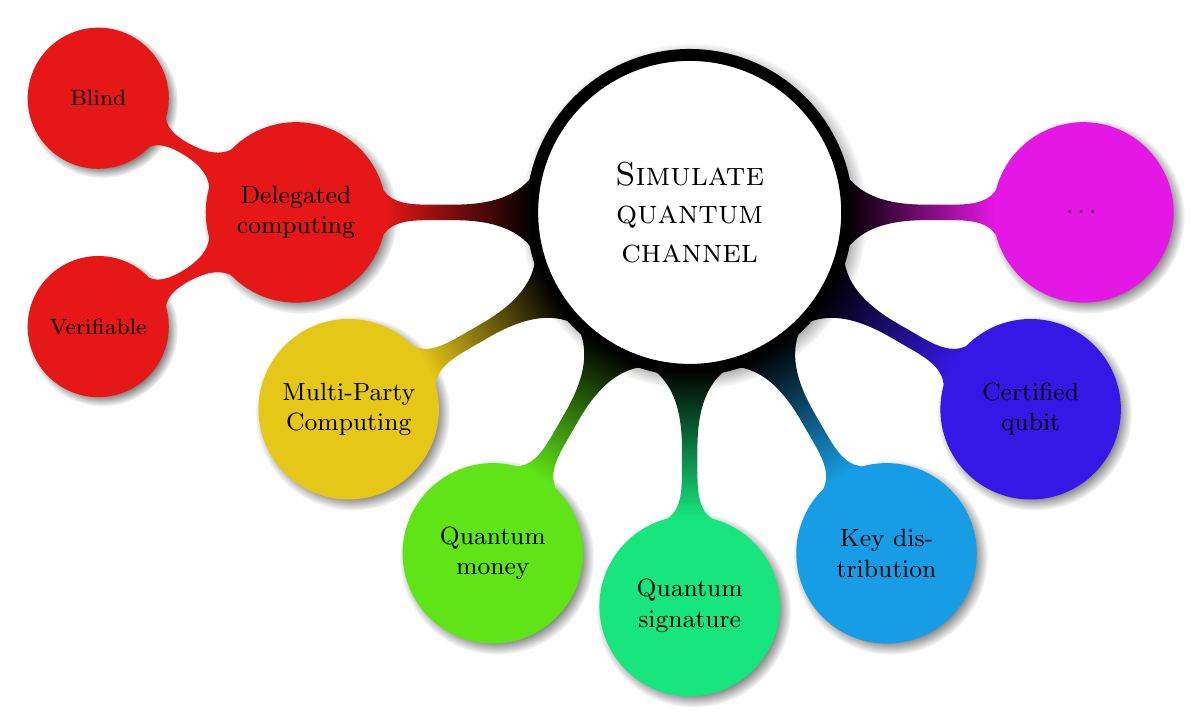
\begin{tikzpicture}[rotate=-90]
        \colorlet{color min hsb}[hsb]{red}
        \colorlet{color max hsb}[hsb]{magenta}
        \def\bl{90}
        \colorlet{colorA}[rgb]{color max hsb!0!color min hsb!\bl!black}
        \colorlet{colorB}[rgb]{color max hsb!17!color min hsb!\bl!black}
        \colorlet{colorC}[rgb]{color max hsb!33!color min hsb!\bl!black}
        \colorlet{colorD}[rgb]{color max hsb!50!color min hsb!\bl!black}
        \colorlet{colorE}[rgb]{color max hsb!67!color min hsb!\bl!black}
        \colorlet{colorF}[rgb]{color max hsb!83!color min hsb!\bl!black}
        \colorlet{colorG}[rgb]{color max hsb!100!color min hsb!\bl!black}

        % \colorlet{colorA}[rgb]{color max hsb!0!color min hsb!\bl!black}
        % \colorlet{colorB}[rgb]{color max hsb!20!color min hsb!\bl!black}
        % \colorlet{colorC}[rgb]{color max hsb!40!color min hsb!\bl!black}
        % \colorlet{colorD}[rgb]{color max hsb!60!color min hsb!\bl!black}
        % \colorlet{colorE}[rgb]{color max hsb!80!color min hsb!\bl!black}
        % \colorlet{colorF}[rgb]{color max hsb!100!color min hsb!\bl!black}

        \path[mindmap,
          every node/.style={concept, circular drop shadow,execute at begin node=\hskip0pt},
          concept color=black,text=black,font=\bfseries,
          grow cyclic,
          root concept/.append style={
            concept color=black, fill=white, line width=1ex, text=black,
            font=\large\scshape},
          level 1 concept/.append style={sibling angle=180/6}]
        
        node[concept, root concept] {Simulate quantum channel}
        child[concept color=colorA] {
          node[concept] {Delegated computing}
          child { node[concept] {Blind} }
          child { node[concept] {Verifiable} }
        }  
        child[concept color=colorB] {
          node[concept] {Multi-Party Computing}
        }
        child[concept color=colorC] {
          node[concept] {Quantum money}
        }
        child[concept color=colorD] {
          node[concept] {Quantum signature}
        }
        child[concept color=colorE] {
          node[concept] {Key distribution}
        }
        child[concept color=colorF] {
          node[concept] {Certified qubit}
        }
        child[concept color=colorG] {
          node[concept] {\dots}
        };
      \end{tikzpicture}
    }
  \end{figure}
\end{frame}

\subsection{UBQC in a nutshell}

\begin{frame}{UBQC in a nutshell}
  \begin{figure}[ht]
    \centering
    \includepdfpages{figures/slides_ubqc_nutshell/slides_ubqc_nutshell.pdf}
  \end{figure}
\end{frame}

\begin{frame}{UBQC in a nutshell}
  \begin{figure}[ht]
    \centering
        \includepdfpages{figures/slides_ubqc_nutshell/slides_ubqc_nutshell_alice_bob.pdf}
  \end{figure}
\end{frame}

\section{QFactory}

\subsection{Description of the QFactory gadget}

%same comment about the drawing here
\begin{frame}{QFactory: description}
  \begin{figure}[ht]
    \centering
    \includepdfpages{figures/slides_qfactory/replacement.pdf}
    \caption{QFactory gadget: simulate quantum channel}
  \end{figure}
\end{frame}


\begin{frame}{QFactory: description}
  \begin{figure}[ht]
    \centering
    \includepdfpages{figures/slides_qfactory/ideal_functionality.pdf}
    \caption{QFactory: ideal functionality}
  \end{figure}
\end{frame}

\subsection{Cryptographic assumptions}

\begin{frame}{Cryptographic assumptions}
  \begin{figure}[ht]
    \centering
    \includepdfpageswidth{\linewidth}{figures/slides_qfactory/cryptographic_assumptions.pdf}
  \end{figure}
\end{frame}
%I think we were using "One-way"
%I would suggest either changing the post quantum description to "Hard to invert even against quantum computers" or combining it with the one-wayness
%Either "Funtions {f_k}" or "family function {f_k}"
\subsection{Construction}

% I think the symbol for measurements has an arrow at the end :p, also maybe we can use the same symbol for M_{alpha_i} and just add the angle as opposed to 0/1 meas

\begin{frame}[t]{Construction}%
  \vspace{-4mm}%
  \begin{columns}
    \column{\dimexpr\paperwidth-10pt}
    \begin{figure}[ht]
      \centering
      \includepdfpageswidth{1\textwidth}{figures/slides_qfactory/protocol_explanation.pdf}
      % TODO: enlarge the slide and remove margins
    \end{figure}
  \end{columns}
\end{frame}

\section{Security}

\subsection{Hidden GHZ State and $\theta$}
\begin{frame}[t]{Hidden GHZ State and $\theta$}
  \begin{figure}[ht]
    \centering%
    \foreach \x in {1,2,3,4}{%
      \only<\x>{\includegraphics[width=.6\textwidth]{figures/ghz_\x.pdf}}%
    }%
  \end{figure}
\end{frame}

\begin{frame}{Intuition security}
  TODO: Intuition security, PostBQP...
\end{frame}

\subsection{Hardcore function and Honest-but-curious model}
\begin{frame}[t]{Hardcore function and Honest-but-curious model}
  \begin{columns}
    \begin{column}{.5\textwidth}
    \begin{figure}[ht]
      \centering
      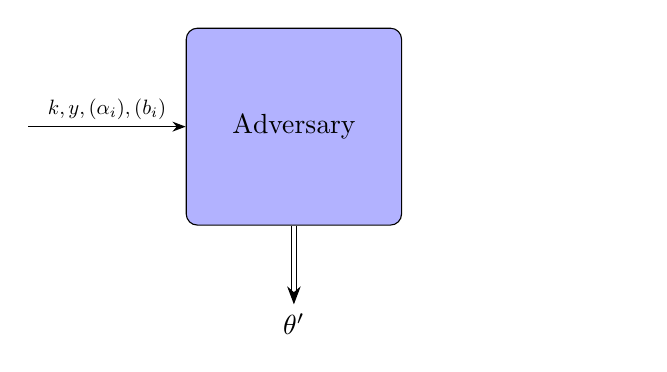
\begin{tikzpicture}
        \node[draw,rectangle,rounded corners,align=center,text width=2.5cm,minimum height=2.5cm,fill=blue!30] (adv) {Adversary};
        \coordinate (m) at ($(adv.north west)!.5!(adv.south west)$);
        \draw[arrows = {-Stealth[scale=1]}] ([xshift=-2cm]m) -- (m)
        node[midway,above,scale=.75] (ky) {$k,y,(\alpha_i),(b_i)$};
        \draw[arrows = {-Stealth[scale=1]}, double distance=1.5pt] (adv.south) -- ([yshift=-1cm]adv.south)
        node[below] {$\theta'$};
        % Center the picture
        % \coordinate () at ;
        \path[] (adv.north east) -- ([xshift=3cm]adv.north east);
      \end{tikzpicture}%
    \end{figure}
    Cannot be better than random guess: $\theta$ \textbf{hardcore} function.
  \end{column}%
  % 
  \begin{column}{.5\textwidth}
    \begin{exampleblock}{Honest-but-curious model}
      Corollary: secure in the
      honest-but-curious model.\\
      If adversary:
      \begin{itemize}
      \item follows the protocol
      \item can only access classical registers
      \end{itemize}
      $\Rightarrow $ he cannot guess $\theta$
    \end{exampleblock}
  \end{column}
\end{columns}
\end{frame}

%TODO I would suggest adding one slide with the construction(s) of the function as well, maybe also say a bit about MP11

%TODO For the hardcore function slide, maybe we can also write a definition of hardcore or an intuition on why theta should be hardcore (given the GL theorem)

%TODO In the summary I would write more applications that might attract the audience, basically rewriting the applications from your drawing because now it should be clearer after seeing the construction on how QFactory could be used in all these settings

% TODO: Add slides to answer questions
% TODO: Compare work Urmila
\section{}
\begin{frame}{Summary and future work}
  \begin{block}{Summary}
    \begin{itemize}
    \item QFactory: simulate quantum channel from classical channel
    \item \tcancel{quantum client} $\rightarrow$ classical clients:\\Applications: classically driven (verifiable) blind quantum computing\dots
    \item For now, proof in honest-but-curious model
    \end{itemize}
  \end{block}
  \begin{exampleblock}{Future work}
    \begin{itemize}
    \item Improve proof of security in Universal Composability model
    \item Improve efficiency in blind computing
    \item Explore new possible applications, certified qubits (QFactory + Zero Knowledge proof) that could improve MPC\dots
    \end{itemize}
  \end{exampleblock}
\end{frame}

\begin{frame}{Questions}
  \begin{figure}[ht]
    \centering
    Thank you for your attention!\\
    Any question?
    %% TODO: not beautifull
  \end{figure}
\end{frame}

\end{document}

%%% Local Variables:
%%% mode: latex
%%% TeX-master: t
%%% End:
